\documentclass[preview,border=5pt]{standalone}
\usepackage{teaching}
\begin{document}

\centering

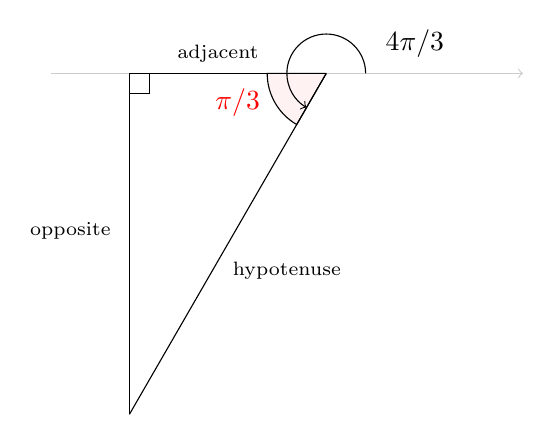
\begin{tikzpicture}[yscale=1,xscale=1,scale=5,inner sep=0.3mm, label distance=1.5mm]

\draw [->,color=black!20!white] (-0.7,0) -- (0.5,0);
%\draw [->,color=black!20!white] (0,-1.2) -- (0,1.2);
%\node(1) at (1.25,0) [color=black!20!white] {$x$};
%\node(2) at (0,1.25) [color=black!20!white] {$y$};
%\node(0) at (-0.1,-0.1) [color=black!20!white] {$0$};
%\draw[black!20!white] (0,0) -- (1.1,1.90525588833);
%\draw[black!20!white] (-1.1,1) -- (2,1);
%\draw[black!20!white] (1,-1.1) -- (1,1.9);

%\draw[fill=fgold!10!white,fill opacity=0.5] (0,0) -- (0.2,0) arc (0:30:0.2cm)  -- (0,0);
%\draw (0,0) -- (0.86602540378,0.5);
%\draw[color=fgold!50!white, dashed] (0.86602540378,0.5) -- (0.86602540378,0);
%\draw[color=fgold!50!white, dashed] (0.86602540378,0.5) -- (0,0.5);
%\node(t) at (0.86602540378,-0.075) [color=fgold] {$\sqrt{3}/2$};
%\node(t) at (-0.1,0.5) [color=fgold] {$1/2$};

%\draw[fill=blue!10!white,fill opacity=0.5] (0,0) -- (0.15,0) arc (0:60:0.15cm)  -- (0,0);
%\draw (0,0) -- (0.5,0.86602540378);
%\draw[color=blue!50!white, dashed] (0.5,0) -- (0.5,0.86602540378);
%\draw[color=blue!50!white, dashed] (0,0.86602540378) -- (0.5,0.86602540378);
%\node(t) at (0.5,-0.075) [color=blue] {$1/2$};
%\node(t) at (-0.12,0.86602540378) [color=blue] {$\sqrt{3}/2$};

\draw[fill=red!10!white,fill opacity=0.5] (0,0) -- (-0.15,0) arc (180:240:0.15cm)  -- (0,0);
\draw (0,0) -- (-0.5,-0.86602540378);
\draw (-0.5,0) -- (-0.5,-0.86602540378);
\draw (0,0) -- (-0.5,0);
\draw[->] (0.1,0) arc (0:240:0.1cm);

%\node(t) at (0.12,-0.86602540378) [color=red] {$\sqrt{3}/2$};
%\node(t) at (-0.5,0.075) [color=red] {$1/2$};

%\node(t) at (0.3,0.075) [color=fgold] {$\pi/6$};
%\node(t) at (0.18,0.175) [color=blue] {$\pi/3$};
\node(t) at (-0.225,-0.075) [color=red] {$\pi/3$};
\node(t) at (0.225,0.075) {$4\pi/3$};
\node(t) at (-0.275,0.05) {\scriptsize adjacent};
\node(t) at (-0.65,-0.4) {\scriptsize opposite};
\node(t) at (-0.1,-0.5) {\scriptsize hypotenuse};

\draw (-0.5,0) -- (-0.5,-0.05) -- (-0.45,-0.05) -- (-0.45,0);

%\node(t) at (1.05,-0.05) [color=black!50!white] {$1$};
%\node(t) at (-1.075,-0.05) [color=black!50!white] {$-1$};
%\node(t) at (-0.05,1.05) [color=black!50!white] {$1$};
%\node(t) at (-0.075,-1.075) [color=black!50!white] {$-1$};

%\draw (-1,1.73205080757) -- (2.2,-0.11547005383);
%\draw[thick,red] (0.5,0) -- (0.5,0.86602540378);
%\node(B) at (0.675,0.4) [red] {$\sin\theta$};
%\draw[thick,blue] (0,0.86602540378)--(0.5,0.86602540378);
%\node(C) at (0.25,0.8) [blue] {$\cos\theta$};
%\draw[thick,purple] (0,0) -- (2,0);
%\node(D) at (1.5,-0.1) [purple] {$\sec\theta$};
%\draw[thick,orange] (0,0) -- (0,1.15470053838);
%\node(E) at (-0.175,0.575) [orange] {$\csc\theta$};
%\draw[thick,cyan] (0.5,0.86602540378) -- (2,0);
%\node(F) at (1.25,0.6) [cyan] {$\tan\theta$};
%\draw[thick,magenta] (0,1.15470053838) -- (0.5,0.86602540378);
%\node(G) at (0.4,1.1) [magenta] {$\cot\theta$};

%\draw (0,0) circle (1);

\end{tikzpicture}

\end{document}